   %%%%%%%%%%%%%%%%%%%
   %                 %
   %  capitolo2.tex  %
   %                 %
   %%%%%%%%%%%%%%%%%%%

\chapter{Un caso storico: i kaoni neutri}
\section{I kaoni}
\noindent
I kaoni $K^0$, $K^+$, $K^-$ e $\bar{K}^0$ sono quattro mesoni appartenenti a quello che oggi viene detto \emph{ottetto dei mesoni pseudoscalari}, insieme ai pioni
ed alla particella $\eta$. 
In Tab.\ref{quattrokaoni} sono riassunte brevemente le caratteristiche principali dei quattro kaoni.
\begin{table}
\begin{center}
\begin{tabular}{|c|c|c|c|c|c|}\hline
Autostato di \emph{flauvor} & Quark componenti & $J^P$ & Stranezza & $I_3$ & $Q$\\\hline
$K^-$ & $\bar{u}s$ & $0^-$ & $-1$ & $-1/2$ & $-e$\\\hline
$\bar{K}^0$ & $\bar{d}s$ & $0^-$ & $-1$ & $+1/2$ & $0$\\\hline
$K^0$ & $d\bar{s}$ & $0^-$ & $+1$ & $-1/2$ & $0$\\\hline
$K^+$ & $u\bar{s}$ & $0^-$ & $+1$ & $+1/2$ & $+e$\\\hline
\end{tabular}
\end{center}
\caption{Caratteristiche principali dei quattro kaoni. Si è indicata con $Q$ la carica elettrica (espressa come multiplo della carica del
positrone) con $I_3$ la terza componente dell'isospin e con $J^P$ lo spin - parità.}
\label{quattrokaoni}
\end{table}

La scoperta dei kaoni risale al 1947, quando G. D. Rochester e C. C. Butler, dell'università di Manchester, studiando le tracce prodotte in una camera a nebbia dai 
raggi cosmici a bassa quota, osservarono una coppia di tracce cariche che si allontanavano formando una figura a forma di V. Queste vennero interpretate come
il risultato del decadimento in volo di una nuova particella neutra, la cui massa venne stimata pari a circa mille masse
elettroniche. Oggi questa particella è nota con il nome di $K_S$ e risulta essere, come verrà discusso più avanti, un autostato di propagazione dato 
da una sovrapposizione di $K^0$ e $\bar{K}^0$ \cite{Kabir}.
L'importanza storica dei kaoni è dovuta al fatto che furono le prime particelle scoperte dotate del numero quantico della \emph{stranezza}, che venne
introdotto proprio ai tempi delle prime osservazioni per spiegare alcuni aspetti del comportamento delle nuove particelle che risultavano appunto, secondo la fisica 
del tempo, strani. Ad esempio, non era chiaro perché i kaoni, benché venissero prodotti da reazioni veloci, su scale di tempo tipiche delle interazioni forti 
($\approx 10^{-23}$ secondi) presentassero vite medie di durata tipica delle interazioni deboli ($\approx 10^{-10}$, $10^{-8}$ secondi)\cite{Krane}.
I kaoni sembravano inoltre poter essere creati soltanto in coppie, ad esempio secondo la reazione:
\begin{equation}\label{Kaone1}
 \pi^- + p \longrightarrow n + K^- + K^+
\end{equation}
oppure, al più, insieme ad altre particelle strane, come la $\Lambda$, ad esempio secondo la reazione:
\begin{equation}\label{Kaone2}
 \pi^- + p \longrightarrow \Lambda + K^0
\end{equation}
La \emph{stranezza} venne introdotta proprio per superare queste difficoltà. Essa fu originariamente definita in funzione della carica elettrica, della terza componente 
dell'isospin e del numero barionico $B$ \cite{Kabir}:
\begin {equation}\label{stranezza}
S = 2(Q - I_3 - \frac{B}{2})
\end{equation}
Si suppose che questa quantità dovesse essere necessariamente conservata dalle interazioni forti, inibendo di fatto un eventuale decadimento forte dei kaoni.
Nel Modello Standard, nel quale gli adroni risultano essere composti da quark, la stranezza è una caratteristica propria del quark $s$, che in base alla 
definizione originaria \eqref{stranezza} ha stranezza pari a $-1$ mentre il suo antiquark $\bar{s}$ ha stranezza $+1$.
Si può facilmente verificare che le reazioni \eqref{Kaone1} e \eqref{Kaone2}, nelle quali interviene la forza forte, conservano la stranezza ($K^+$ e $K^0$ hanno stranezza pari 
a $+1$, $K^-$ e $\Lambda$ pari a $-1$).
\begin{figure}
\begin{center}
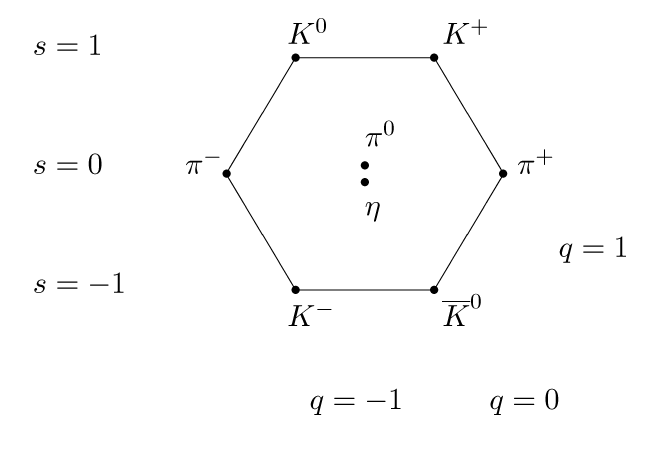
\includegraphics[scale=1]{Immagini/Meson_octet}
\caption{Gli otto mesoni dell'\emph{ottetto pseudoscalare}. Di ciascuno viene indicata la carica elettrica e la stranezza.}
\end{center}
\end{figure}

Nel seguito verrà trattato principalmente il comportamento dei kaoni neutri $K^0$ e $\bar{K}^0$, che presentano una serie di effetti quantomeccanici di notevole interesse.
Si tratta di particelle instabili, che condividono gli stessi canali di decadimento:
\begin{center}
\begin{tabular}{ll}
$K^0$ & $\rightarrow \pi^+ \pi^-$\\
 & $\rightarrow \pi^0 \pi^0$\\
 & $\rightarrow \pi^0 \pi^0 \pi^0$\\
 & $\rightarrow \pi^0 \pi^+ \pi^-$\\
 & $\rightarrow \pi^{\pm} \mu^{\mp} \nu_{\mu} (\bar{\nu_{\mu}})$\\
 & $\rightarrow \pi^{\pm} e^{\mp} \nu_{e} (\bar{\nu_{e}})$
\end{tabular}
\end{center}
\begin{center}
\begin{tabular}{ll}
$\bar{K^0}$ & $\rightarrow \pi^+ \pi^-$\\
 & $\rightarrow \pi^0 \pi^0$\\
 & $\rightarrow \pi^0 \pi^0 \pi^0$\\
 & $\rightarrow \pi^0 \pi^+ \pi^-$\\
 & $\rightarrow \pi^{\pm} \mu^{\mp} \nu_{\mu} (\bar{\nu_{\mu}})$\\
 & $\rightarrow \pi^{\pm} e^{\mp} \nu_{e} (\bar{\nu_{e}})$
\end{tabular}
\end{center}
Ciò, come verrà esposto nelle sezioni successive, è alla base del peculiare comportamento del sistema $K^0$ - $\bar{K}^0$. 

\section{Oscillazioni di stranezza}
\noindent
L'evoluzione temporale di un sistema di kaoni neutri presenta un effetto che non ha eguali in nessun altro tipo di sistema fisico (fatta eccezioni per i mesoni $D^0$, $B^0$ e 
$B_s$, che presentano notevoli analogie con i $K^0$): la trasformazione di una particella nella propria antiparticella.
Ciò è dovuto al fatto che $K^0$ e $\bar{K^0}$ non sono stati indipendenti ma possono oscillare l'uno nell'altro attraverso processi deboli virtuali intermedi del secondo ordine, ad esempio:
\begin{equation}
 K^0 \leftrightarrow \pi \pi \leftrightarrow \bar{K}^0
\end{equation}
Come risultato di questo accoppiamento, un fascio inizialmente puro di kaoni $K^0$ può essere osservato, ad un istante successivo, come miscela $K^0$ - $\bar{K}^0$.
Ne consegue che gli autostati di sapore $K^0$ e $\bar{K}^0$ non rappresentano la base più adatta per uno studio del sistema $K^0$ - $\bar{K}^0$ e, poiché ai tempi della scoperta
si credeva che ogni interazione dovesse conservare CP, venne naturale studiare tale sistema in funzione degli autostati di $\mathscr{C}\mathscr{P}$, $K_1$ e $K_2$:
\begin{equation}\label{K1}
|K_1\rangle=\frac{1}{\sqrt{2}} (|K^0\rangle + |\bar{K}^0\rangle)
\end{equation}
\begin{equation}\label{K2}
|K_2\rangle=\frac{1}{\sqrt{2}} (|K^0\rangle - |\bar{K}^0\rangle)
\end{equation}
Si verifica facilmente che:
\begin{equation}
 \mathscr{C}\mathscr{P}|K_1\rangle = |K_1\rangle
\end{equation}
\begin{equation}
\mathscr{C}\mathscr{P}|K_2\rangle = -|K_2\rangle 
\end{equation}
A questo punto, è necessario verificare il comportamento sotto $\mathscr{C}\mathscr{P}$ dei canali di decadimento, al fine di verificare quali di essi abbiano $CP = 1$
e quali $CP = -1$. Poiché, dal punto di vista sperimentale, lo studio dei decadimenti adronici è più agevole di quello relativo ai decadimenti semileptonici, ci si limiterà
a discutere i primi. Si considera dapprima il comportamento sotto $\mathscr{C}$ e $\mathscr{P}$ di un singolo pione. Valgono le seguenti relazioni:
\begin{equation}
 \mathscr{C}\psi(\pi^\pm) \rightarrow \psi(\pi^\mp)
\end{equation}
\begin{equation}
 \mathscr{C}\psi(\pi^0) \rightarrow \psi(\pi^0)
\end{equation}
\begin{equation}
 \mathscr{P}\psi(\pi) \rightarrow -\psi(\pi)
\end{equation}
dove, nell'ultima equazione, si è indicato con $\pi$ uno qualsiasi dei pioni $\pi^0$, $\pi^+$ o $\pi^-$, mentre il segno meno è dovuto al fatto che i pioni hanno parità 
intrinseca negativa. Dalle considerazioni appena fatte segue che, nel caso di sistema di due pioni si ha:
\begin {equation}
\mathscr{C}\mathscr{P}|\pi\pi\rangle = \mathscr{P}\mathscr{C}|\pi\pi\rangle = \mathscr{P}|\pi\pi\rangle = (-1)^2 (-1)^l |\pi\pi\rangle = |\pi\pi\rangle
\end{equation}
Nell'ultimo passaggio si è tenuto conto del fatto che i kaoni $K^0$ e $\bar{K}^0$ (quindi anche gli autostati di $\mathscr{C}\mathscr{P}$ $K_1$ e $K_2$) hanno spin 0 e quindi 
la conservazione del momento angolare impedisce ai prodotti di decadimento di avere momento angolare orbitale reciproco.
Quindi se ne conclude che:
\begin{equation}
 \mathscr{C}\mathscr{P}|\pi,\pi\rangle = |\pi,\pi\rangle
\end{equation}
Allo stesso modo, è possibile verificare che:
\begin{equation}
 \mathscr{C}\mathscr{P}|\pi,\pi,\pi\rangle = -|\pi,\pi,\pi\rangle
\end{equation}
In base al ragionamento fin qui fatto, i due autostati di $\mathscr{C}\mathscr{P}$ $K_1$ e $K_2$, devono decadere rispettivamente in due ed in tre pioni.
Quindi ci si attende che $K_2$ abbia una vita media sensibilmente più lunga del $K_1$, in quanto la maggior differenza di massa tra stati iniziali e stati 
finali favorisce il decadimento di quest'ultimo.

Le osservazioni sperimentali evidenziarono appunto, all'interno di un fascio di kaoni $K^0$ o $\bar{K}^0$, la presenza di due stati distinti, uno a vita media più breve,
per questo battezzato $K_S$ (\emph{K short}) ed uno a vita media più lunga, $K_L$ (\emph{K long}).
Le prime osservazioni sembrarono anche confermare il fatto che i decadimenti in due pioni erano caratteristici del $K_S$, mentre quelli in tre pioni del $K_L$, dando
un'importante conferma alla teoria del miscelamento dei kaoni $K^0$ e $\bar{K}^0$ negli autostati di CP chiamata anche, dai nomi dei due fisici che per primi la proposero,
\emph{teoria di Gell-Mann Pais}\cite{Kabir}. 

\section{Rigenerazione}
\noindent
Poiché le reazioni solitamente usate per la produzione di $K^0$:
\begin{equation}
 \pi^- + p \rightarrow \Lambda^0 + K^0
\end{equation}
\begin{equation}
 \pi^0 + n \rightarrow \Lambda^0 + K^0
\end{equation}
hanno una sezione d'urto significativa, si deduce, a causa del Teorema CPT, che i due processi:
\begin{equation}
\bar{K}^0 + p \rightarrow \Lambda^0 + \pi^+
\end{equation}
\begin{equation}
\bar{K}^0 + n \rightarrow \Lambda^0 + \pi^0
\end{equation}
debbano avere anch'essi una notevole sezione d'urto, così come le reazioni a queste simili nelle quali $\Lambda^0$ è sostituito da un iperione $\Sigma$. 
Ciò equivale a dire che i $\bar{K}^0$ reagiscono violentemente con la materia nucleare, dalla quale vengono assorbiti. 
Al contrario, i $K^0$ interagiscono molto più debolmente, spesso attraverso semplici urti elastici, risultando quasi completamente inerti.
Se si assume la validità della teoria di \emph{Gell-Mann Pais}, l'evoluzione di un sistema di kaoni neutri può essere descritta in termini dei due autostati di $\mathscr{CP}$, 
$K_S$ (il kaone neutro a vita breve) e $K_L$ (il kaone neutro a vita media lunga).

Si definiscono $\tau_S$ e $\tau_L$ le vite medie dei due stati, con $\tau_S << \tau_L$.
Un fascio di $K^0$ inizialmente puro, dopo un tempo $\tau$ tale per cui $\tau_S << \tau << \tau_L$, risulterà composto quasi esclusivamente da $K_L$:
\begin{equation}
 |K_L\rangle = \frac{1}{\sqrt{2}}\big(|K^0\rangle - |\bar{K}^0\rangle\big)
\end{equation}
mentre l'autostato $K_S$ potrà, sotto ogni aspetto pratico, essere considerato assente.
Ora si ponga sulla traiettoria del fascio un materiale di spessore tale che, nell'attraversamento di questo da parte dei $K_L$, si abbia una probabilità di interazione
da parte di un $\bar{K}^0$ prossima ad $1$. Questo materiale è, per i $\bar{K}^0$, qualcosa che approssima molto bene un assorbitore ideale, mentre i $K^0$ vengono trasmessi
senza attenuazioni. Il sistema, che era stato osservato come uno stato puro $K_L$ a monte dell'assorbitore, risulta quindi essere uno stato puro $K^0$ a valle di questo.
Ma questo ragionamento era iniziato appunto considerando un fascio puro di $K^0$, per cui si può iterare quanto detto finora e riesprimere questo come una sovrapposizione
$K_S$ e $K_L$. Il passaggio attraverso l'assorbitore ha quindi \emph{rigenerato} la componente $K_S$. 

Questo fenomeno, studiato e riprodotto sperimentalmente per la
prima volta da Pais e Piccioni, rappresenta una delle prime prove sperimentali della teoria del miscelamento tra gli autostati di sapore per opera dell'interazione debole \cite{Kabir}.

\section{Violazione di CP}
\begin{figure}
\begin{center}
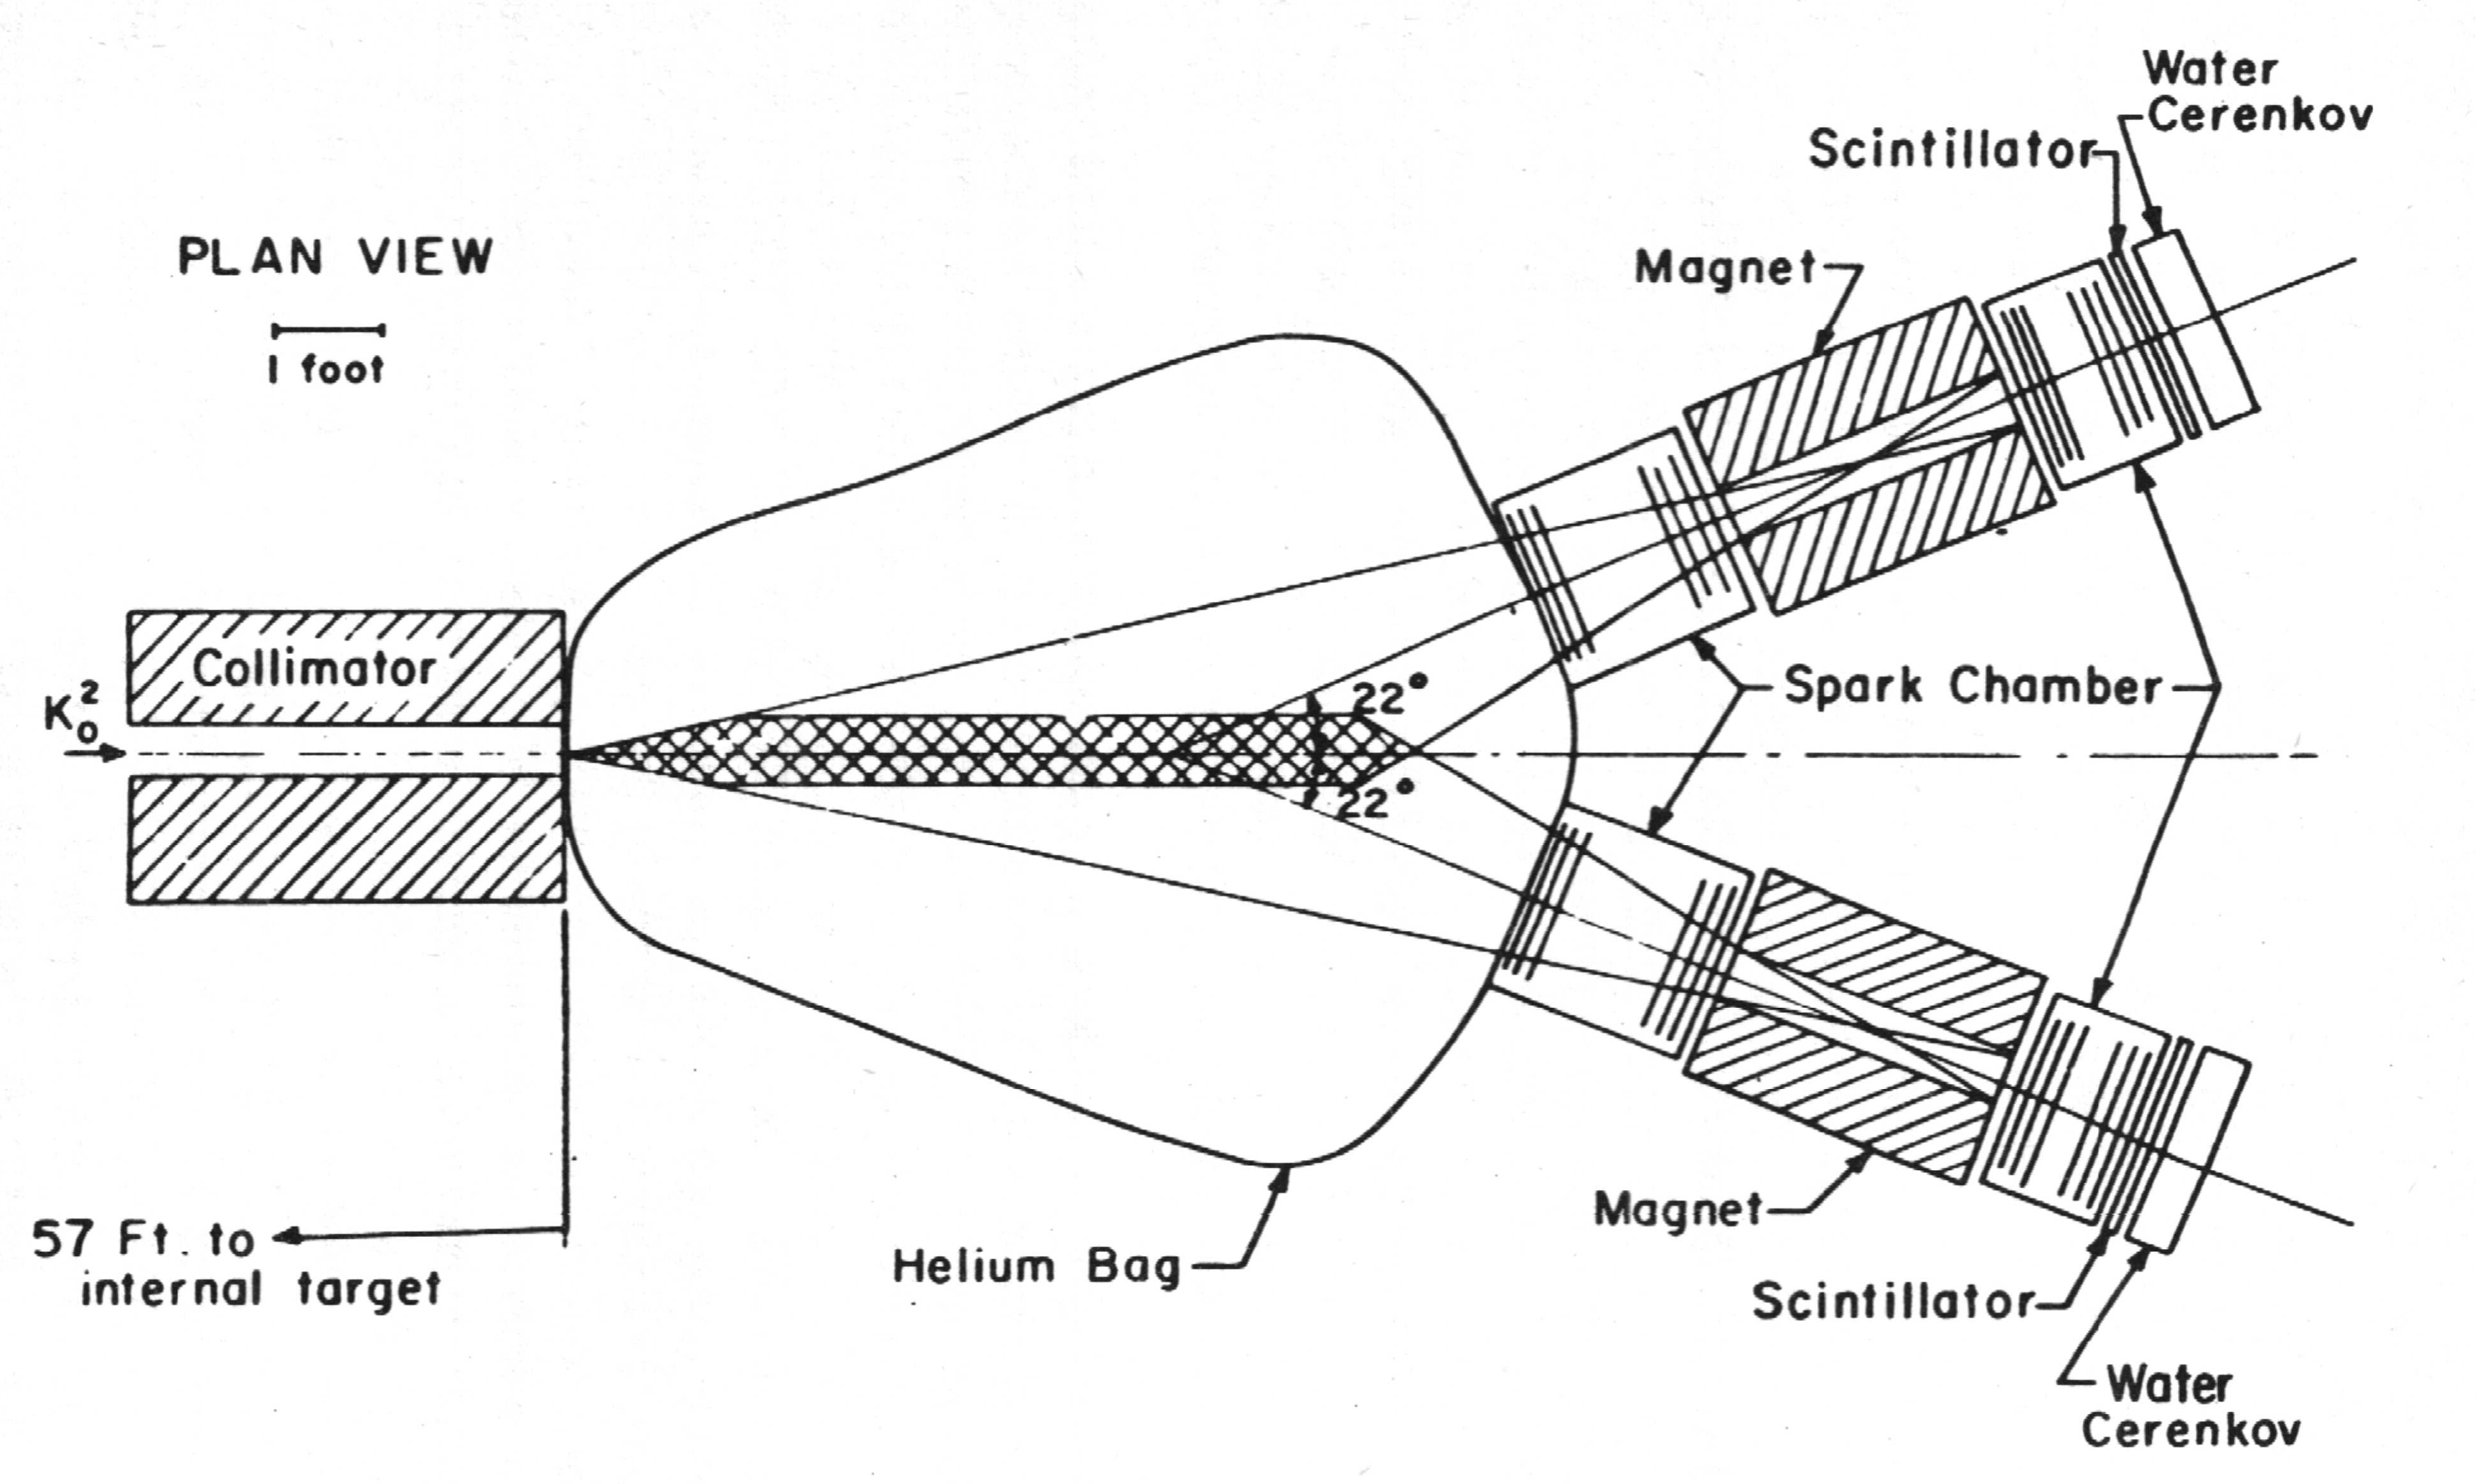
\includegraphics[scale=0.1]{Immagini/rilevatore}
\caption{Schema dell'apparato sperimentale impiegato da  Christenson, Cronin, Fitch e Turlay per l'osservazione del decadimento $K_L \longrightarrow \pi^+ \pi^-$}
\end{center}
\end{figure}
\noindent
Nel luglio del 1964 Christenson, Cronin, Fitch e Turlay annunciarono la sconcertante scoperta del decadimento:
\begin{equation}\label{CPviolation}
 K_L \longrightarrow \pi^+ \pi^-
\end{equation}
L'esperimento da loro allestito al Brookhaven National Laboratory, negli Stati Uniti, consisteva nel far percorrere ad un fascio di $K^0$ una distanza tale che la 
componente $K_S$ che raggiungeva il rilevatore fosse trascurabilmente piccola, quindi si studiavano i canali di decadimento del $K_L$.
Il canale \eqref{CPviolation} risultava avvenire con un \emph{branching ratio} pari a circa $0,3\%$, segno che nella dinamica del sistema $K^0$-$\bar{K}^0$
doveva esserci una violazione di CP a livello dello $0,3\%$ \cite{Krane}. 
Esattamente venne misurato il rapporto:
\begin{equation}
\frac{\Gamma (K_L\rightarrow \pi\pi)}{\Gamma (K_L\rightarrow all)} = (2,3 \pm 0,3) × 10^{−3}
 \end{equation}
In questo caso si parla di violazione di CP nel \emph{mixing}.
Un secondo metodo che venne proposto per testare la violazione di CP da parte del sistema dei kaoni neutri fu il confronto dei $rates$ di decadimenti
CP-coniugati, ad esempio:
\begin{equation}
 K_L \longrightarrow \pi^- \mu^+ \bar{\nu}_{\mu}
\end{equation}
\begin{equation}
 K_L \longrightarrow \pi^+ \mu^- \nu_{\mu}
\end{equation}
Se CP fosse una simmetria esatta i $rates$ dei due decadimenti dovrebbero essere identici, invece sperimentalmente questi risultarono differenti, 
ancora una volta di circa lo $0,3\%$, confermando il fatto che il sistema non fosse CP-invariante. In questo caso si parla di violazione di CP diretta \cite{Wong}.

A causa della violazione di CP, si dedusse anche che gli autostati di propagazione libera $K_L$ e $K_S$ non coincidono esattamente con gli autostati di CP $K_1$ e 
$K_2$ definiti dalle \eqref{K1} e \eqref{K2}, ma che fossero una sovrapposizione di entrambi:
\begin{equation}
    K_L = \frac{K_2 + \epsilon_1 K_1}{\sqrt{1+|\epsilon_1|^2}}  
\end{equation}
\begin{equation}
    K_S = \frac{K_1 + \epsilon_2 K_2}{\sqrt{1+|\epsilon_2|^2}}  
\end{equation}
dove $\epsilon_1$ ed $\epsilon_2$ sono due numeri complessi, che per il teorema CPT devono essere uguali ed il cui modulo è di ordine di grandezza pari all'entità di
violazione di CP ($\approx 10^{-3}$). \cite{Lee}

Per la scoperta della violazione di CP nel sistema $K^0$-$\bar{K}^0$, Cronin e Fitch ricevettero il Premio Nobel per la Fisica nel 1980.
